% This is part of Un soupçon de mathématique sans être agressif pour autant
% Copyright (c) 2015
%   Laurent Claessens
% See the file fdl-1.3.txt for copying conditions.

\begin{exercice}\label{exo2smath-0255}

    Le but de cet exercice est de montrer que les formules de distribution et de factorisation fonctionnent \emph{vraiment} pour toutes les valeurs «des lettres».

    \begin{enumerate}
        \item   \label{ItemFSHZooXBKFIk}
            Sur papier : développer et réduire : \( 3\times (x+3)-x\).
        \item
            Avec un tableur, pour une vingtaine de valeurs de \( x\) entre \( -10\) et \( 10\), faire calculer les valeurs de \( 3(x+3)-x\) ainsi que de votre résultat à la question \ref{ItemFSHZooXBKFIk}. Que remarquez-vous ?
        \item
            Quel est le problème avec ce tableau ?

            \begin{center}
            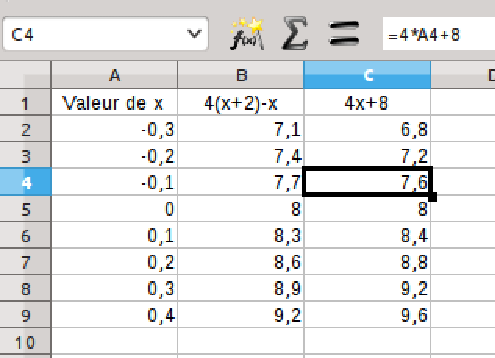
\includegraphics[width=5cm]{faux_tableur.pdf} 
            \end{center}

    \end{enumerate}
    
\corrref{2smath-0255}
\end{exercice}
